\chapter{Calibration}
\label{sec:calibration}

\cleanchapterquote{If you want to know the value of a security, use the price of another security that is as similar to it as possible. All the rest is modelling.}{Emanuel Derman}{(1946)}

In order to be able to price a FX-TARN, we have to calibrate our models to the market option prices. The aim of the calibration is to estimate the unknown parameters of the model which reproduce the same prices as in the market. This is analogous to the implied volatility in the Black-Scholes framework. For this purpose, we will use European vanilla option prices calculated from the implied volatility given by \textsc{Bloomberg}.

Firstly, in Section \ref{sec:calibration:inputs}, we will present the calibration inputs and how we can compute the European vanilla option price. Secondly, in Section \ref{sec:calibration:method}, we will explain the procedure that we used to calibration our models. In Section \ref{sec:calibration:results}, we will discuss about the results of the calibrations of our models. The Section \ref{sec:calibration:analysis} concludes this chapter with the analysis of the resulting calibrated models.

\section{Calibration inputs}
\label{sec:calibration:inputs}
All the data we have used in this chapter come from the provider \textsc{Bloomberg}. We have recovered the implicit volatility quotes with respect to the delta Call or delta Put and tenor for the exchange rate USD/CHF on the 23 May 2017. The delta notations are listed in the Table \ref{tab:delta} with the corresponding theoretical delta. 

\begin{table}[!ht]
\centering
  \begin{tabular}{c|c||c|c}
   \toprule
   Notation & Delta & Notation & Delta\\
   \toprule
   5D Put & -0.05  & 5D Call  & 0.05\\ 
   10D Put & -0.10 & 10D Call & 0.10\\
   15D Put & -0.15 & 15D Call & 0.15\\
   25D Put & -0.25 & 25D Call & 0.25\\
   35D Put & -0.35 & 35D Call & 0.35\\
   \bottomrule
  \end{tabular}
  \vspace{5pt}
  \caption{\label{tab:delta} Notation convention of delta Call and delta Put.}
\end{table}
For the calibration, we have only used the volatility quotes for maturities 1W, 2W, 3W, 1M, 2M, 3M, 4M, 6M, 9M and 1Y. At the end, that represents 110 implied volatilities including ATM ($\Delta = \pm 0.50$) quote.

The Figure \ref{fig:calibration:depo} shows us the CHF and USD risk-free rate curves used in our calibration.
\begin{figure}[!htb]
	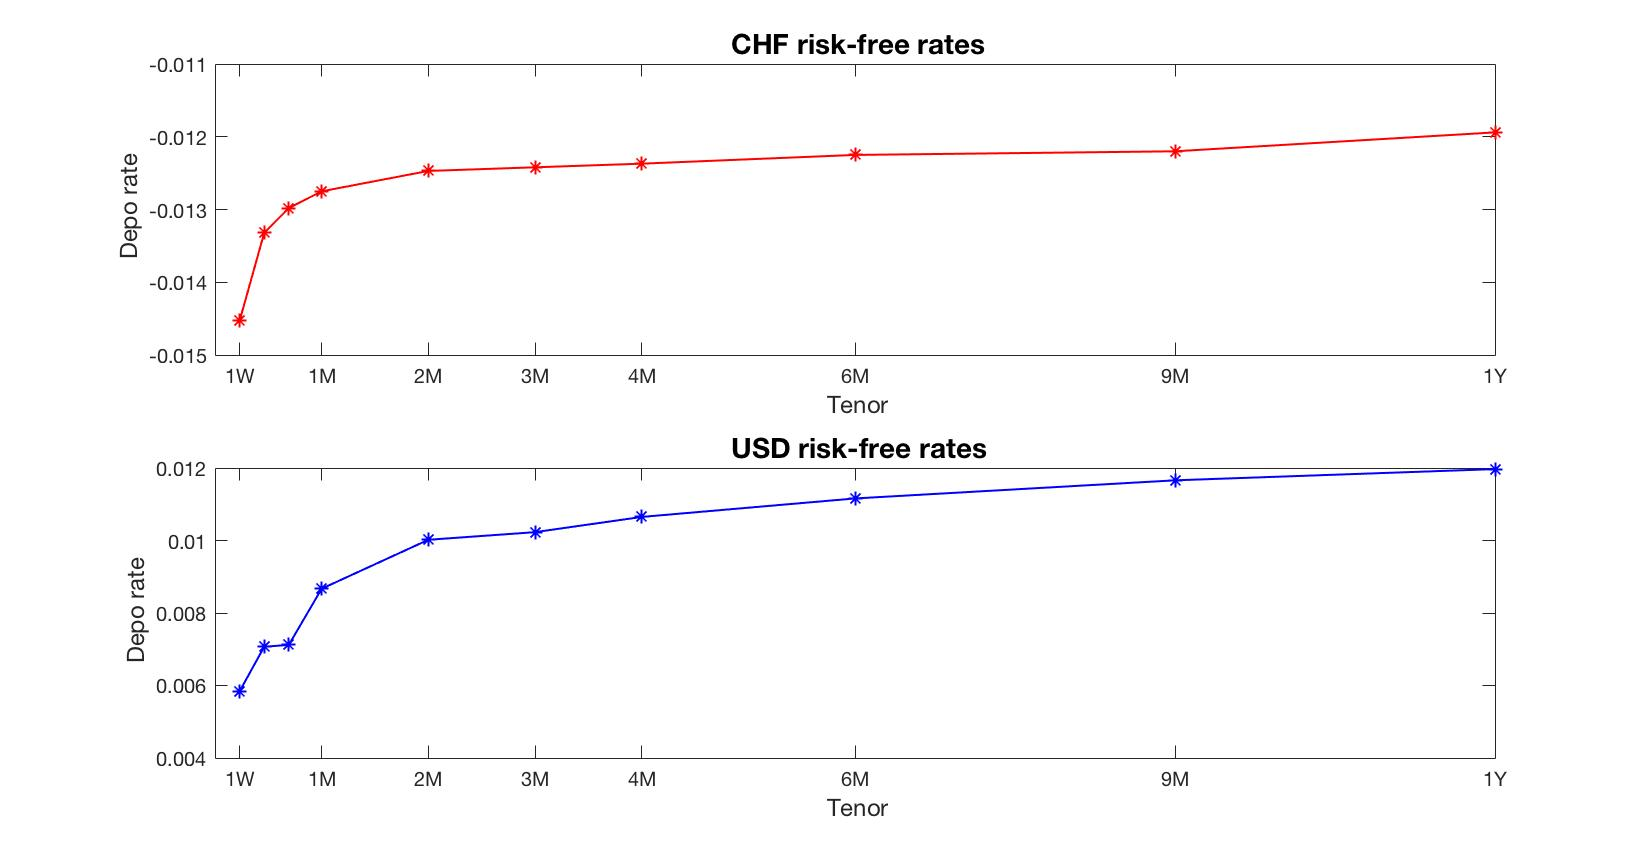
\includegraphics[width=\textwidth]{gfx/risk-free}
	\caption{Risk-free rates from \textsc{Bloomberg} used for the calibration.}
	\label{fig:calibration:depo}
\end{figure}

Since the implied volatilities are quoted with respect to the delta, to compute the European vanilla option price, we have to recover the corresponding strike. In the Black-Scholes framework, we have the following relationship between the delta $\Delta$ and the strike $K$:
$$K = S_0e^{(r_d-r_f)T}  \exp\left(-\beta \sigma \sqrt{T}\Phi^{-1}\left(e^{-r_f T}  |\Delta|\right) + \frac{1}{2} \sigma^2 T\right),
$$
where $\beta = 1$ for a Call option and $\beta = -1$ for a Put option and $\Phi$  is the standard Gaussian cumulative probability function. The initial spot price $S_0 = 0.9730$ is naturally given by the term sheet of the FX-TARN.

From here, we can use the Black-Scholes formula to compute the European vanilla option prices:
$$V(K,T) = \beta\left(S_0 e^{-r_f T}\Phi(\beta d_+)-Ke^{-r_d T}\Phi(\beta d_-)\right),$$
with
$$d_\pm = \frac{\log\left(\frac{S_0e^{(r_d-r_f)T}}{K}\right)\pm \frac{1}{2}\sigma^2 T}{\sigma \sqrt{T}}.$$

The delta less than 50 means that the market quotes are priced with respect to out of the money (OTM) options. Therefore, we have computed the OTM European option prices under Black-Scholes model illustrated in Figure \ref{fig:calibration:prices}. On the left hand side, we have the OTM Put options and on the right hand side, we have the OTM Call options.
\begin{figure}[!htb]
\centering
	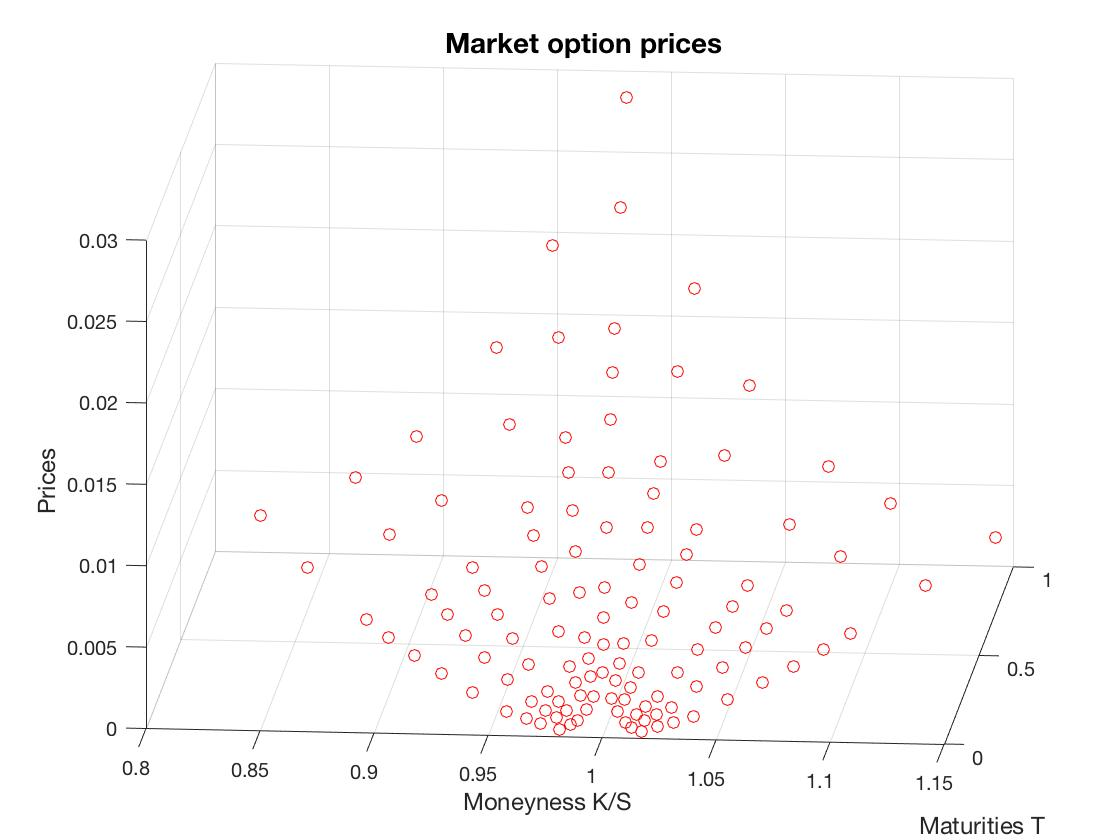
\includegraphics[scale = 0.3]{gfx/Euro-prices}
	\caption{European option prices; on the left hand side, the OTM Put options, and on the right hand side, the OTM Call options.}
	\label{fig:calibration:prices}
\end{figure}

\section{Calibration method}
\label{sec:calibration:method}
To calibrate our models, we seek to minimize the root-mean-square error (RMSE) of the differences between the model prices and the observed prices:
$$\text{RMSE}(\Theta) = \sqrt{\sum_{i=1}^N \frac{1}{N}\left|V(\Theta;K_i,T_i)-V^\text{obs}(K_i,T_i)\right|^2},$$
where $\Theta$ is the parameter vector of the model.

For example, the RMSE of the Black-Scholes model with 1Y ATM constant volatility, $\sigma = 0.07908$, is equal to $8.95\cdot 10^{-4}$, which is not very precise. Effectively, we can observe in the Figure \ref{fig:calibration:BS} that the model prices don't fit good with the market prices. We will see that the jump models perform better than the Black-Scholes model. 
\begin{figure}[!htb]
\centering
	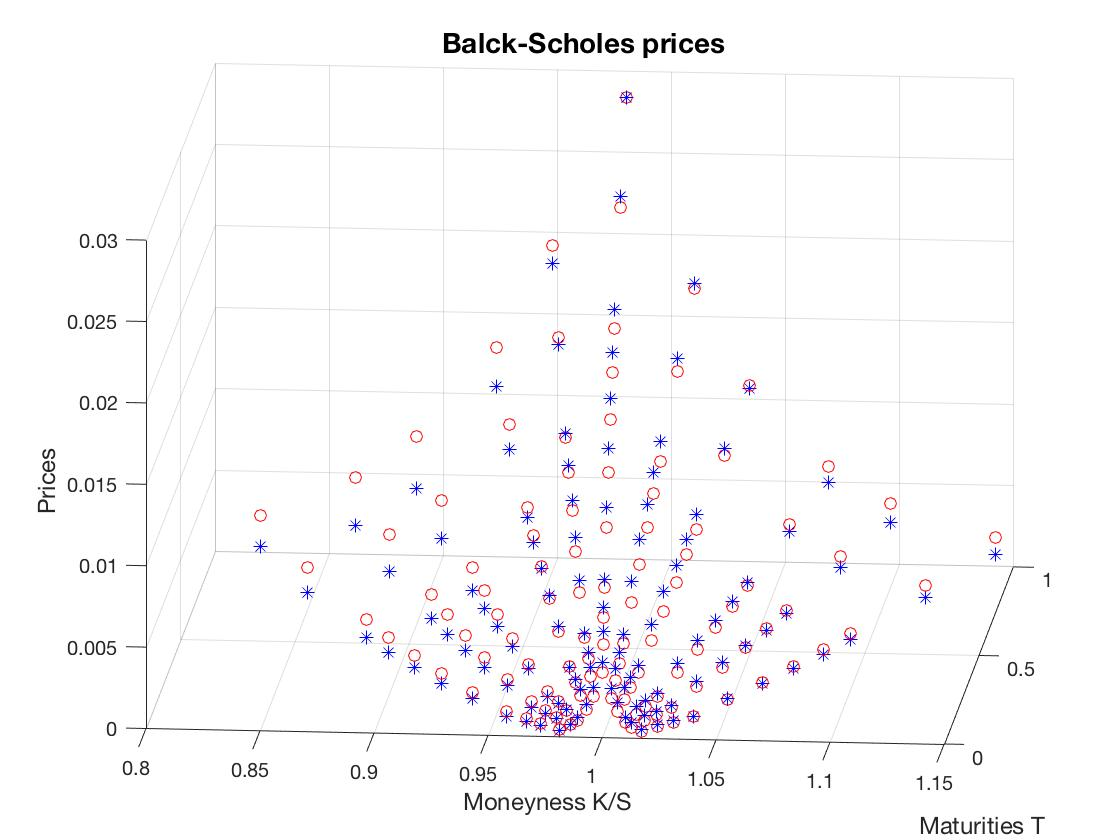
\includegraphics[scale = 0.3]{gfx/BS-prices}
	\caption{Black-Scholes prices (in blue) in comparison with the market prices (in red).}
	\label{fig:calibration:BS}
\end{figure}

The calibrated parameters $\hat{\Theta}$ of the model with jumps satisfy 
$$\hat{\Theta}=\operatorname*{arg\,min}_\Theta \text{RMSE}(\Theta).$$
We can use the \textsc{Matlab} command \texttt{fmincon} which allows us to find the minimum of a constrained nonlinear multi-variable function. Note that the method used to price the European options under jump models is the convolution method with $N_x = 1'000$ and damping factor $\alpha = -\beta$, where $\beta = 1$ for a Call option and $\beta = -1$ for a Put option. This method is in fact the fastest method to apply the minimizing function.

\section{Results of calibrations}
\label{sec:calibration:results}
The resulting calibrated parameters and RMSE for each jumps models are summarized in the the Table \ref{tab:param} in comparison with the Black-Scholes model. We can see that all models perform better that the Black-Scholes model. The models that fit the best the market prices are the jump-diffusion models because they have more parameter and give more freedom in the calibration.
\begin{table}[!ht]
\centering
  \begin{tabular}{l|c|c}
    \toprule
    Models & Calibrated parameters $\hat{\Theta}$ & RMSE \\
    \toprule
   Black-Scholes($\sigma$) & $[0.07908]$ & $8.98\cdot 10^{-4}$ \\
   \midrule
   Merton($\sigma,\lambda,\alpha,\delta$)  & $[0.0649,0.1303,-0.0584,0.1603]$ & $2.77\cdot 10^{-4}$\\
   Kou($\sigma,\lambda,p,\eta_1,\eta_2$) & $[0.0665,0.1305,0.0751,3.3154,9.0490]$&$2.49 \cdot 10^{-4}$ \\
   \midrule
   NIG($\alpha,\beta,\delta$) & $[18.8492,-3.9282,0.1250]$&$4.79\cdot 10^{-4}$\\
   VG($\theta, \sigma,\nu$) & $[-0.0324,0.0810,0.2451]$&$5.73\cdot 10^{-4}$\\
    \bottomrule
  \end{tabular}
  \vspace{5pt}
  \caption{\label{tab:param} Calibrated parameters $\hat{\Theta}$ and RMSE for each models.}
\end{table}
\newpage
We can see in Figure \ref{fig:calibration:jump-prices} that all the model prices are more closed to the market prices than the results obtained with Black-Scholes. This means that the FX-TARN price computed with jump model will be more relevant with respect to the market than the FX-TARN price under Black-Scholes.

\begin{figure}[!htb]
\centering
	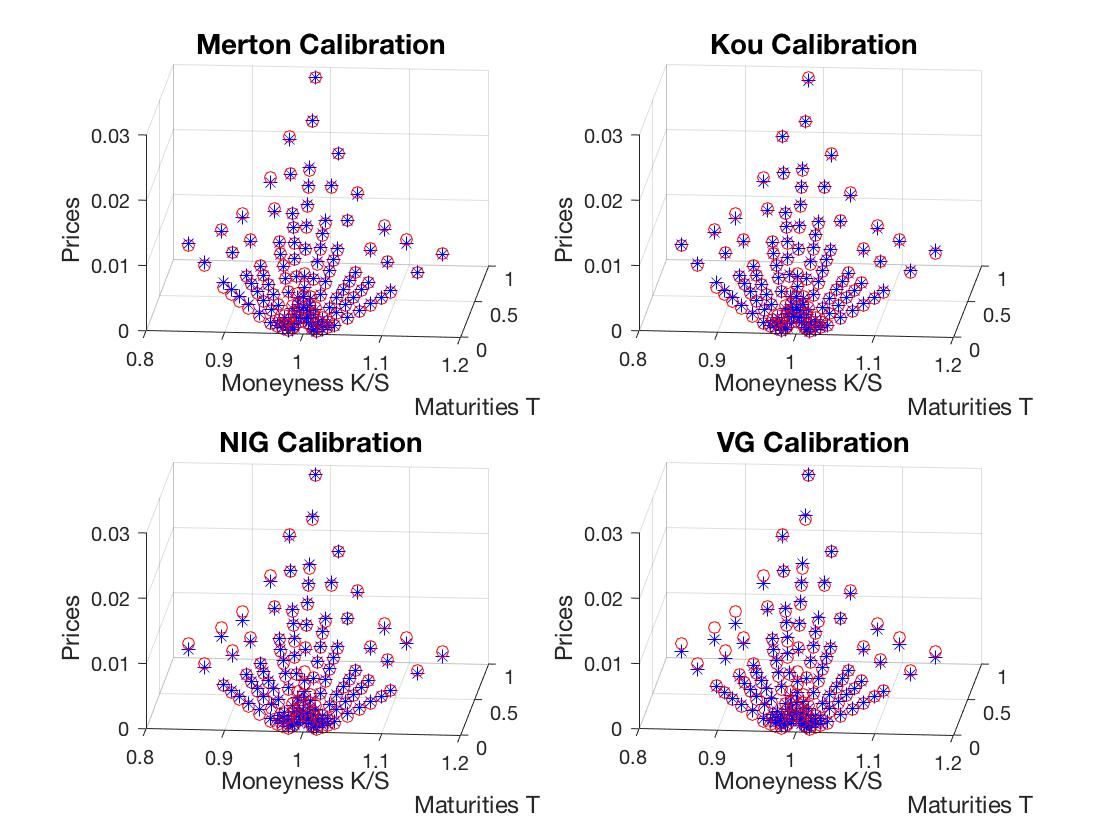
\includegraphics[width=\textwidth]{gfx/Jump-calibration}
	\caption{Jump models calibration; model prices in blue and market prices in red.}
	\label{fig:calibration:jump-prices}
\end{figure}

\section{Analysis of the calibration}
\label{sec:calibration:analysis}
As we have chosen to calibrate our models for whole structure of the implied volatility, i.e. for all tenors at the same time, the fitting with the market prices can not be perfect. We will now investigate how the L\'evy models with jumps reflect the information contained in the smile of the volatility surface. Figure \ref{fig:vol_surf} shows the original volatility surface that we used to calibrate our models.
\begin{figure}[!htb]
\centering
	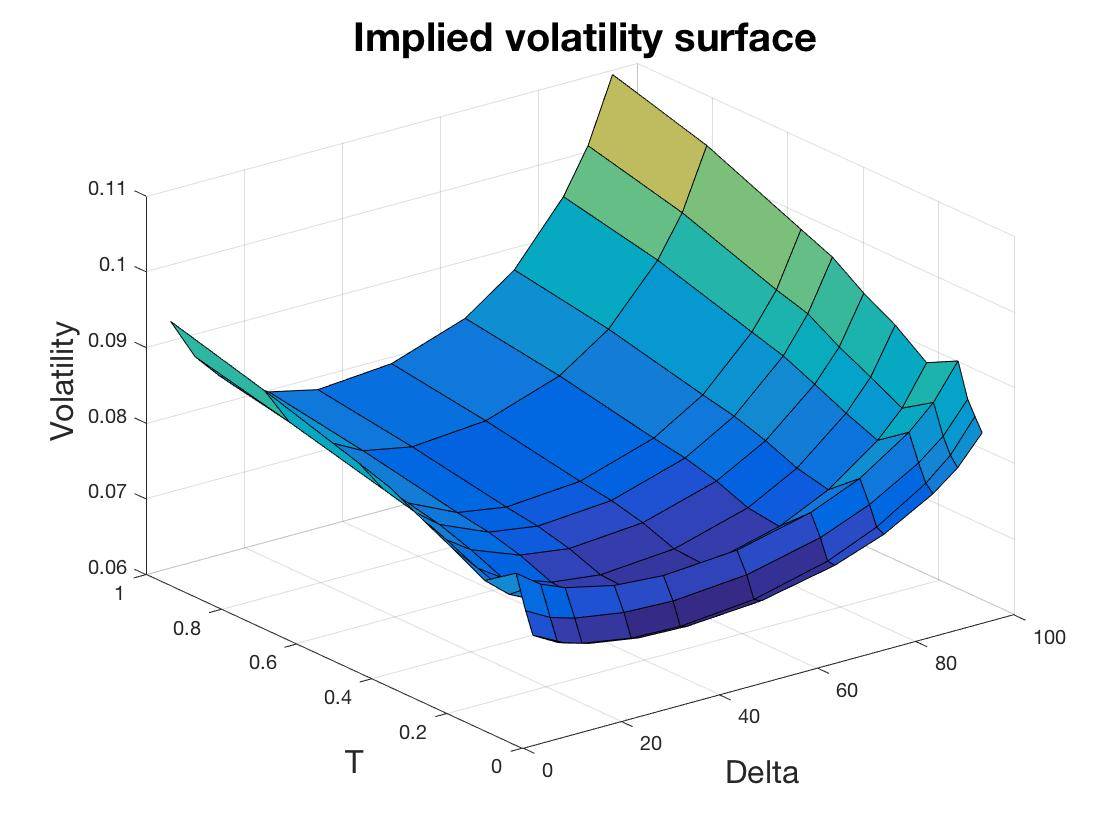
\includegraphics[scale = 0.2]{gfx/vol_surf}
	\caption{Original volatility surface.}
	\label{fig:vol_surf}
\end{figure}

By repricing all the options with the L\'evy models with jumps, it is possible to compute the volatility surface corresponding the a specific model. Figure \ref{fig:vol_models} illustrates the implied volatility surfaces of the L\'evy models with jumps. 
\begin{figure}[!htb]
\centering
	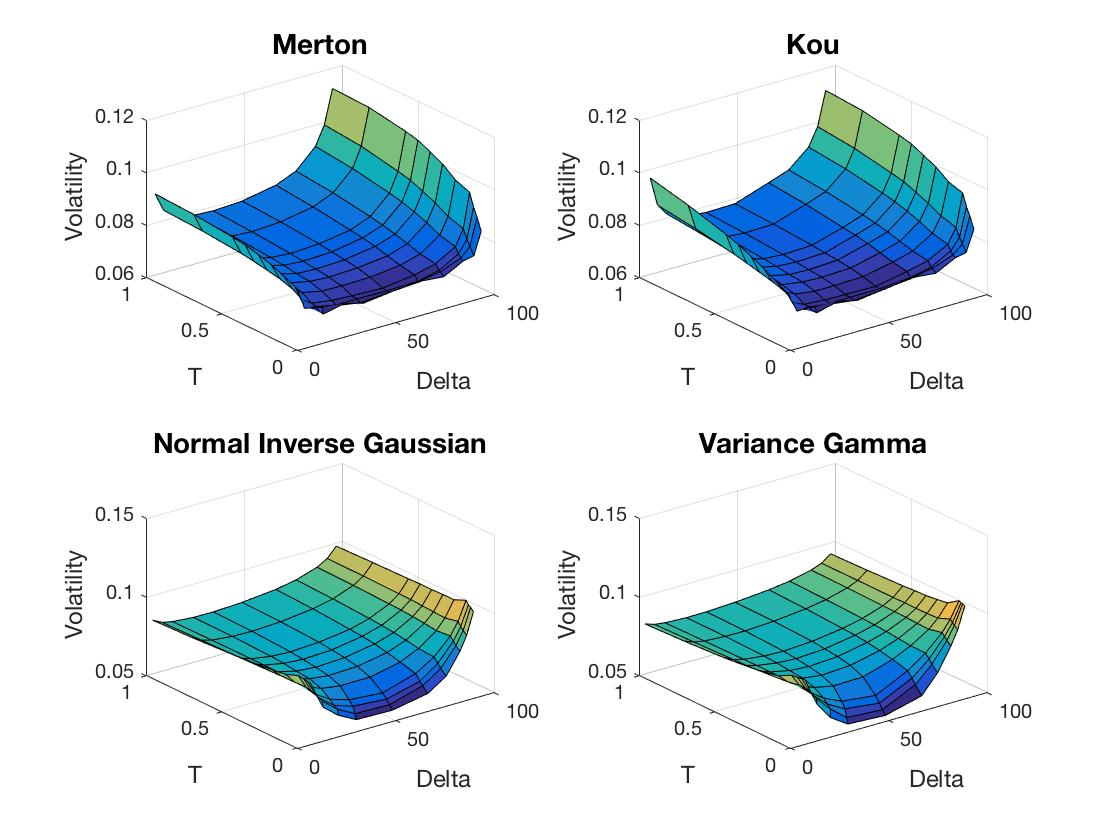
\includegraphics[width=\textwidth]{gfx/vol_models}
	\caption{Jump models implied volatility surfaces.}
	\label{fig:vol_models}
\end{figure}

As we can see, the jump-diffusion models replicate almost the original volatility surface, which means that the Merton and Kou models can express all the information contained in the volatility smile. On the other side, the smile structure in pure jump models for long term is lost. Thus the pure jumps model can not replicate perfectly the market prices for long maturity.

An other way to check the accuracy of the calibration of a model is to price an option out of the sample used for the calibration. In our case, we can price the European options for the tenor 18M and 2Y with the calibrated models on 1W to 1Y, and compare them to the market prices. The results is given by Figures \ref{fig:out_18m} and \ref{fig:out_2y}.

We can conclude that the Merton and Kou models are clearly more accurate than the NIG and VG models with respect to the market. Indeed, we can see that the NIG and VG do not perform very well deep out of the money for long maturity date. Even if the tenor 18M and 2Y are not part of the sample used for calibration, the Merton and Kou models fit really good with the market prices beyond 1Y maturity. All of this confirm the choice to use jump diffusion models in the pricing of FX-TARN product.

\begin{figure}[!htb]
\centering
	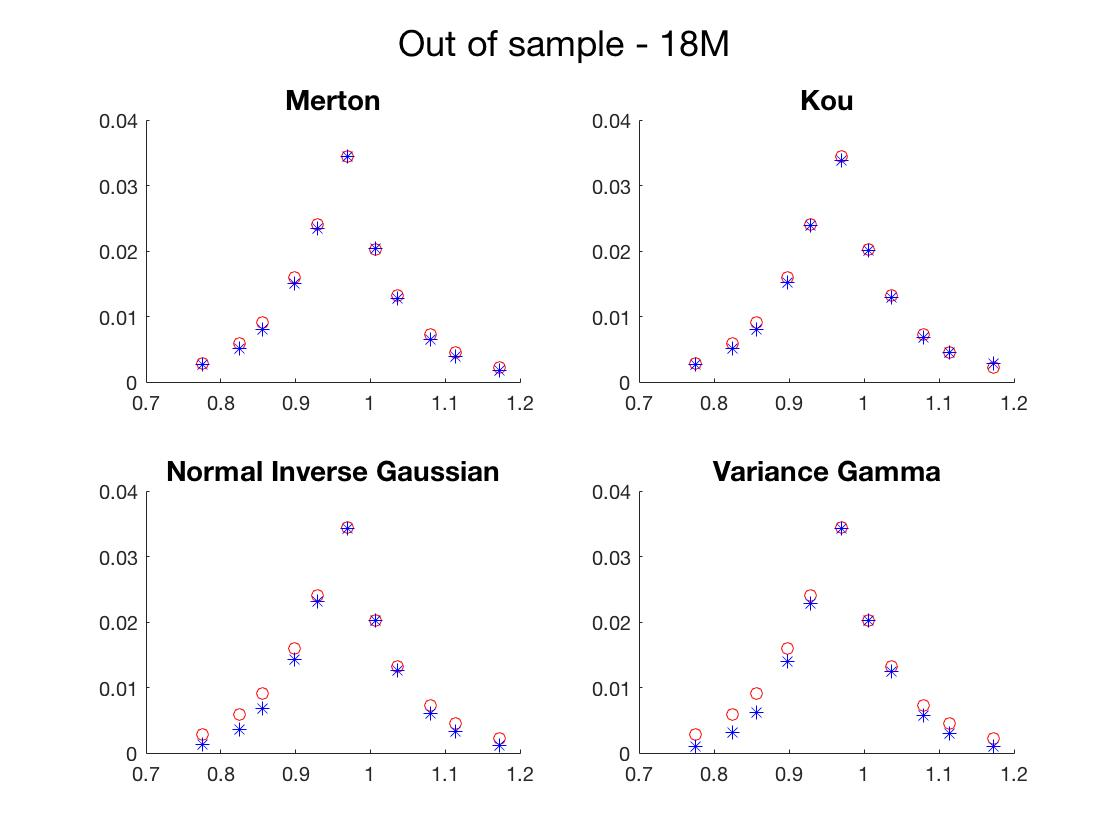
\includegraphics[width=\textwidth]{gfx/out_18m}
	\caption{Out of sample 18M options priced with jump models.}
	\label{fig:out_18m}
\end{figure}
\begin{figure}[!htb]
\centering
	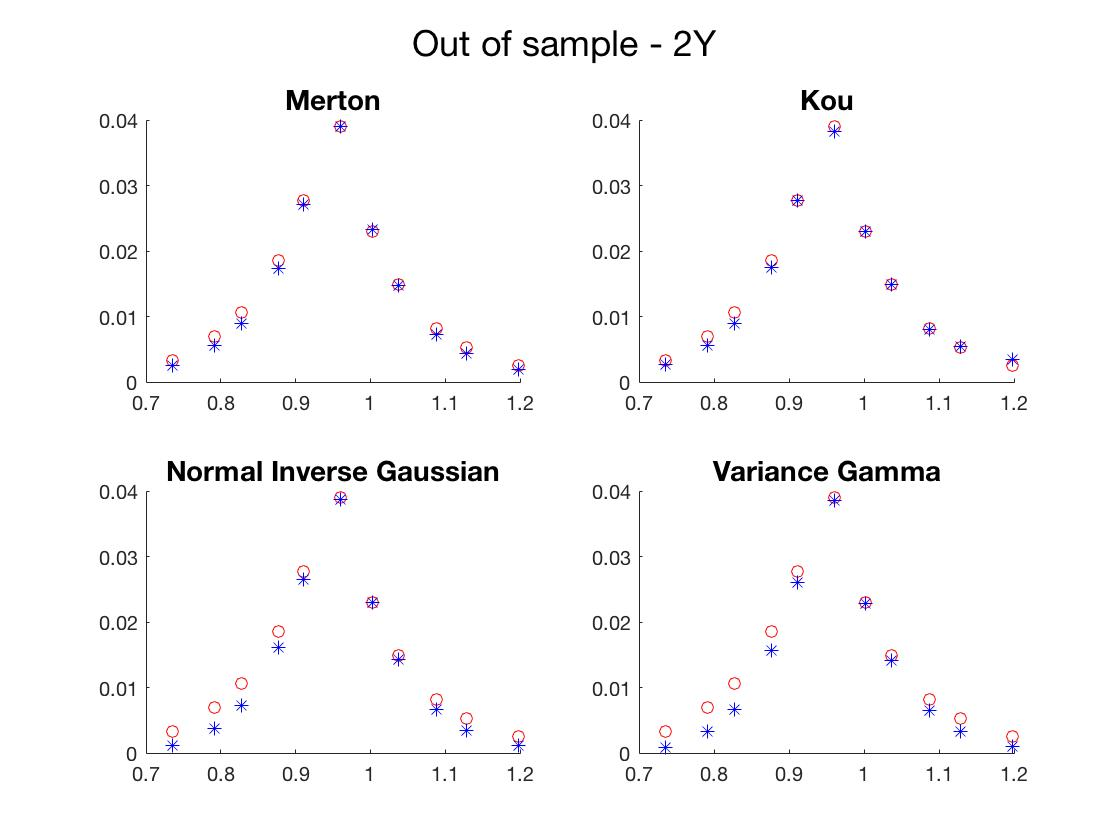
\includegraphics[width=\textwidth]{gfx/out_2y}
	\caption{Out of sample 2Y options priced with jump models.}
	\label{fig:out_2y}
\end{figure}

